% The Word and the Ledger — Verifiable Commitment Provenance for SIGIL, v0.1
% Companion note to SIGIL whitepaper v1. Same house design system.
% Origin: a BitcoinTalk reader (fibonacciopstan) observed that SIGIL gives its
% BINARIES cryptographic provenance while the PROMISES around those binaries have
% none — and asked whether a project built to hold the chain to account can hold
% its own history to account. This note answers: yes, and it is buildable
% precisely because we own the Flux stack from scratch. Honest-status markers and
% future-conditional language enforced. Build: pdflatex x2.
\documentclass[10pt,a4paper]{article}

\usepackage[margin=2.5cm]{geometry}
\usepackage[T1]{fontenc}
\usepackage{lmodern}
\usepackage{amsmath,amssymb,amsfonts}
\usepackage[table]{xcolor}
\usepackage{booktabs}
\usepackage{tabularx}
\usepackage{array}
\usepackage{ragged2e}
\usepackage{enumitem}
\usepackage{microtype}
\usepackage{tikz}
\usetikzlibrary{positioning,arrows.meta}
\usepackage{graphicx}
\graphicspath{{img/}}
\usepackage{tcolorbox}
\tcbuselibrary{skins}
\usepackage{needspace}
\usepackage{fancyhdr}
\usepackage[colorlinks=true,linkcolor=sigilcyan,urlcolor=sigilcyan,citecolor=sigilcyan]{hyperref}
\usepackage{xurl}

% ---------- design system (shared with whitepaper v1) ----------
\definecolor{ink}{HTML}{15171A}
\definecolor{sigilcyan}{HTML}{0086A8}
\definecolor{sigilblue}{HTML}{3B5BDB}
\definecolor{sigilviolet}{HTML}{7048B5}
\definecolor{sigilamber}{HTML}{B86A00}
\definecolor{slate}{HTML}{D7DCE1}
\definecolor{panelbg}{HTML}{F7F7F4}
\definecolor{rowtint}{HTML}{F2F4F6}
\color{ink}

% status markers
\newcommand{\stM}{\textcolor{sigilcyan}{$\bullet$}~{\scriptsize\textcolor{sigilcyan}{\textsc{measured}}}}
\newcommand{\stS}{\textcolor{sigilblue}{$\odot$}~{\scriptsize\textcolor{sigilblue}{\textsc{simulation}}}}
\newcommand{\stG}{\textcolor{sigilviolet}{$\diamond$}~{\scriptsize\textcolor{sigilviolet}{\textsc{staged}}}}
\newcommand{\stO}{\textcolor{sigilamber}{$\circ$}~{\scriptsize\textcolor{sigilamber}{\textsc{open}}}}
\newcommand{\stL}{\textcolor{sigilcyan}{$\bullet$}~{\scriptsize\textcolor{sigilcyan}{\textsc{live}}}}

\newcommand{\layman}[3]{%
\begin{tcolorbox}[enhanced,
  interior style={left color=#1!9,right color=white},
  colframe=#1!45!slate,boxrule=0.5pt,arc=3pt,
  borderline west={2.5pt}{0pt}{#1},
  left=9pt,right=9pt,top=7pt,bottom=7pt]
{\scriptsize\textcolor{#1}{\textsc{in plain words}}\; — \;\textbf{\small #2}}\\[3pt]
\small #3
\end{tcolorbox}}

\widowpenalty=10000
\clubpenalty=10000
\displaywidowpenalty=10000

\pagestyle{fancy}
\fancyhf{}
\fancyhfoffset{0pt}
\renewcommand{\headrulewidth}{0.4pt}
\renewcommand{\headrule}{{\color{slate}\hrule width\headwidth height 0.4pt}}
\fancyhead[L]{\scriptsize\textcolor{gray}{The Word and the Ledger --- verifiable commitment provenance \,$\cdot$\, v0.2}}
\fancyhead[R]{\scriptsize\textcolor{gray}{\thepage}}

\hypersetup{
  pdftitle={The Word and the Ledger — Verifiable Commitment Provenance for SIGIL (v0.2)},
  pdfauthor={bitknight.dipper688@passmail.net},
  pdfsubject={A companion note: extending SIGIL's binary provenance to the project's own promises — roadmap commitments, security disclosures, release announcements, and changes of direction — made content-addressed, hybrid-signed, hash-chained, and anchored on-chain.},
  pdfkeywords={SIGIL, provenance, commitment, accountability, content-addressing, hybrid signatures, transparency log, Flux}
}

\begin{document}

% ---------- title page with braid watermark ----------
\begin{tikzpicture}[remember picture,overlay]
\begin{scope}[shift={(current page.north)},yshift=-4.2cm,opacity=0.065]
  \foreach \yoff/\ph in {0/0, 0.9/2.1, 1.8/4.2}{
    \draw[ink,line width=2.6pt]
      plot[smooth,samples=60,domain=-9:9] (\x,{\yoff-0.9+0.85*cos(60*\x+\ph r)});
  }
\end{scope}
\end{tikzpicture}

\thispagestyle{empty}
\begin{center}
\begin{tikzpicture}
  \node[rounded corners=8pt, fill=ink, inner sep=10pt]
       {
\includegraphics[width=2.2cm]{sigil-flat.png}};
\end{tikzpicture}\\[10pt]
{\Huge\bfseries\textcolor{ink}{The Word and the Ledger}}\\[8pt]
{\Large Verifiable Commitment Provenance for SIGIL}\\[6pt]
{\normalsize A companion note to \emph{SIGIL — The Variational Chain}, whitepaper v1}\\[10pt]
{\normalsize v0.2 · 2026-07-24 · illustrated + external Bitcoin witnessing (\S\ref{sec:time})}\\[6pt]
{\normalsize\texttt{bitknight.dipper688@passmail.net}}\\[2pt]
{\small SIGIL / Flux Foundation · \texttt{sigilgraph.quillon.xyz}}\\[14pt]
\begin{minipage}{0.74\textwidth}
\centering\itshape
``A binary you can verify, wrapped in a promise you cannot, is only half honest.''\\[2pt]
{\upshape\scriptsize --- after a reader's question, this note's origin}
\end{minipage}
\end{center}

\vspace{12pt}

\begin{abstract}
\noindent
SIGIL signs its released binaries with a hybrid post-quantum provenance proof, so
that anyone can check, offline and forever, that a given artifact was attested by a
named key. This note addresses a gap a reader identified: the \emph{promises} around
those binaries --- the roadmap commitments, the security disclosures, the "single
producer today" admissions, the conditions stated as preconditions for mainnet ---
carry no such provenance. GitHub can be reorganized, forum posts edited, websites
and social posts rewritten or deleted. A project whose entire thesis is
\emph{make state divergence explicit and independently checkable} should be able to
make its \emph{own history} explicit and independently checkable by exactly the same
means. We show that this is not an aspiration requiring new cryptography but a direct
composition of primitives SIGIL already ships --- content-addressing, require-both
SQIsign+Ed25519 signatures, an append-only hash chain, and the block header's
event-log commitment --- because the project owns the Flux toolchain end to end. We
define the \emph{Commitment Record}: a content-addressed, hybrid-signed, hash-chained
statement of intent whose digest is anchored in the chain's event-log root, so that a
year later a stranger can prove that a specific promise, in specific words, existed at
a specific block height, signed by a specific key --- and detect, mechanically, any
attempt to quietly rewrite it. We are explicit about scope: this makes a broken or
edited promise \emph{detectable and dated}; it does not, and cannot, force the promise
to be kept. That distinction is the point. The construction is staged, not yet live;
the note itself is offered as the first record the mechanism will anchor.
\end{abstract}

\vspace{6pt}

% ============================================================
\section{The gap a reader found}
% ============================================================
SIGIL's announcement makes many precise, dated, falsifiable statements: that the
network is single-producer today; that the operator can reset or rewrite the chain;
that there is no allocation and no sale; that a named short list of hardening items
gates mainnet; that the post-quantum claim today covers release provenance and
\emph{not} the wallet or consensus signatures. These are exactly the statements that
matter later --- the ones a future observer, or a future version of the project, has an
incentive to soften, reinterpret, or forget.

A reader (\texttt{fibonacciopstan}, on BitcoinTalk) put the problem cleanly: the
released \emph{binaries} carry cryptographic provenance, but the \emph{promises}
surrounding them have none. Repositories can be reorganized or replaced; roadmaps and
websites can be updated; forum posts can be edited; announcements can disappear. So:
\emph{how does someone verify, a year from now, that these were the original
commitments?} And --- the sharper form --- for a project built around holding the chain
to account, shouldn't the community be able to hold the \emph{project's own history}
to account?

\layman{sigilcyan}{the one-sentence version}{We can prove a downloaded program is the
one we signed. We could not, until now, prove that a promise we made last year hasn't
been quietly reworded since. This note fixes the second half with the same tools that
fixed the first.}

We think the observation is correct, and that it exposes an asymmetry worth closing
rather than a rhetorical gotcha to deflect. The rest of this note is the answer.

\begin{figure}[h]
\centering
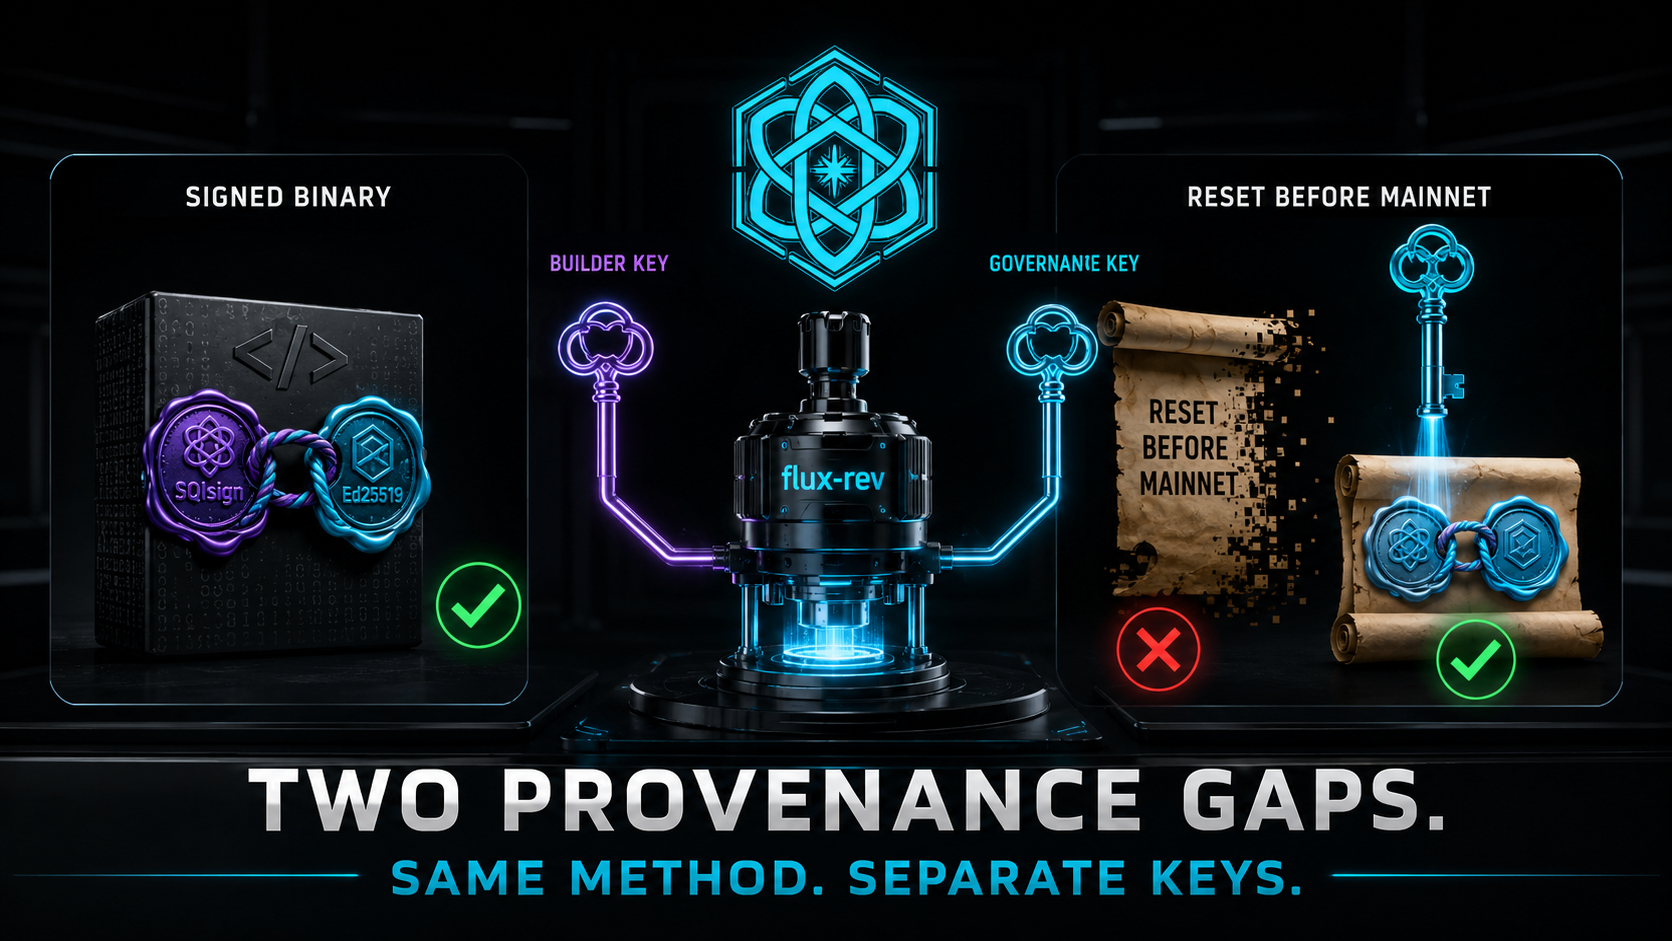
\includegraphics[width=0.94\textwidth]{pro1.png}
\caption{\small The two provenance gaps, closed by the same key. A released binary
carries a require-both seal (verifiable, \textcolor{sigilcyan}{$\checkmark$}); the
promise around it carries none (silently editable, $\times$). The same signer
(\texttt{flux-rev} / require-both) that attests the artifact attests the words --- one
key, two things worth proving.}
\end{figure}

% ============================================================
\section{Why a provenance chain owes this to itself}
% ============================================================
SIGIL's core mechanism is \emph{fail-closed recomputation}: a node commits four
domain-separated state roots per block and halts rather than serve a state whose root
it cannot reproduce (whitepaper v1, \S state commitments). The philosophy companion
frames the whole system as an \emph{epistemic instrument} --- a machine that makes
claims explicit, types their evidence, and refuses authoritative service when local
verification fails.

Turn that instrument on the project itself and the demand is symmetric. A chain that
says \emph{do not trust my ledger, recompute it} has no principled ground to say
\emph{but do trust my roadmap, I remember it correctly}. The credibility of the first
statement is undermined by the ungrounded authority of the second. If divergence in
\emph{money} must be structurally impossible to hide, then divergence between
\emph{what was promised and what is now claimed to have been promised} should be
structurally impossible to hide too --- or the honesty is selective, applied where it
is cheap and withheld where it might one day be inconvenient.

This is not a new principle; it is the transparency-log idea (Certificate
Transparency, binary transparency, Sigstore/Rekor) applied to a project's declarative
statements rather than its certificates or artifacts. What is specific to SIGIL is
that the anchor need not be a third-party log we ask others to trust: it can be
\emph{our own chain}, whose whole reason to exist is to be an append-only,
independently recomputable record.

% ============================================================
\section{The primitives already exist (because we built the stack)}
% ============================================================
The reason this is a composition and not a research program is that owning the Flux
toolchain from the compiler up means every ingredient is already in hand and already
exercised on shipped artifacts:

\begin{itemize}[leftmargin=1.2em,itemsep=3pt]
\item \stL~\textbf{Content-addressing.} \texttt{flux-rev} produces a BLAKE3
  \texttt{full:} identity over a byte set; the download manifest is BLAKE3
  content-addressed. A statement's bytes get a canonical, collision-resistant name.
\item \stL~\textbf{Hybrid post-quantum signing.} The release provenance is a
  \emph{require-both} SQIsign Level 5 \emph{and} Ed25519 attestation over a canonical
  record; a stripped single-leg bundle is rejected, and \texttt{fluxc verify-proof}
  checks both against pinned builder keys. The same signer signs a promise as readily
  as it signs a binary.
\item \stL~\textbf{An append-only hash chain.} SIGIL is, definitionally, a chain of
  per-block commitments folded back to genesis; the light client recomputes the tip
  fingerprint in microseconds. It is already the anchor we need.
\item \stL~\textbf{A header commitment with a home for arbitrary events.} Every block
  header carries an \emph{event-log root} --- a Merkle root over typed events emitted
  that block. On \texttt{sigil-g0} today it commits the canonical empty root
  (\stO~unexercised), but the mechanism that would carry a commitment event is the
  same one already producing the header field.
\item \stL~\textbf{A constant-size prefix proof.} The fold compresses the chain prefix
  to a fixed 2{,}568 bytes; a commitment anchored below the fold horizon inherits a
  succinct existence proof \emph{for free}, verifiable on a light client.
\end{itemize}

Nothing below invents a primitive --- and this is the place to be careful: owning the
Flux stack from scratch is what makes every ingredient \emph{already in hand}, but it
does not, by itself, make the result more \emph{trustworthy}. Building your own tools
strengthens nothing on its own. The trust comes from careful composition,
canonicalization, \emph{data availability}, and --- the point of \S\ref{sec:time} ---
\emph{independent witnessing}. The contribution here is naming the record, fixing its
canonical form, and specifying the verification a stranger runs a year later.

\begin{figure}[h]
\centering
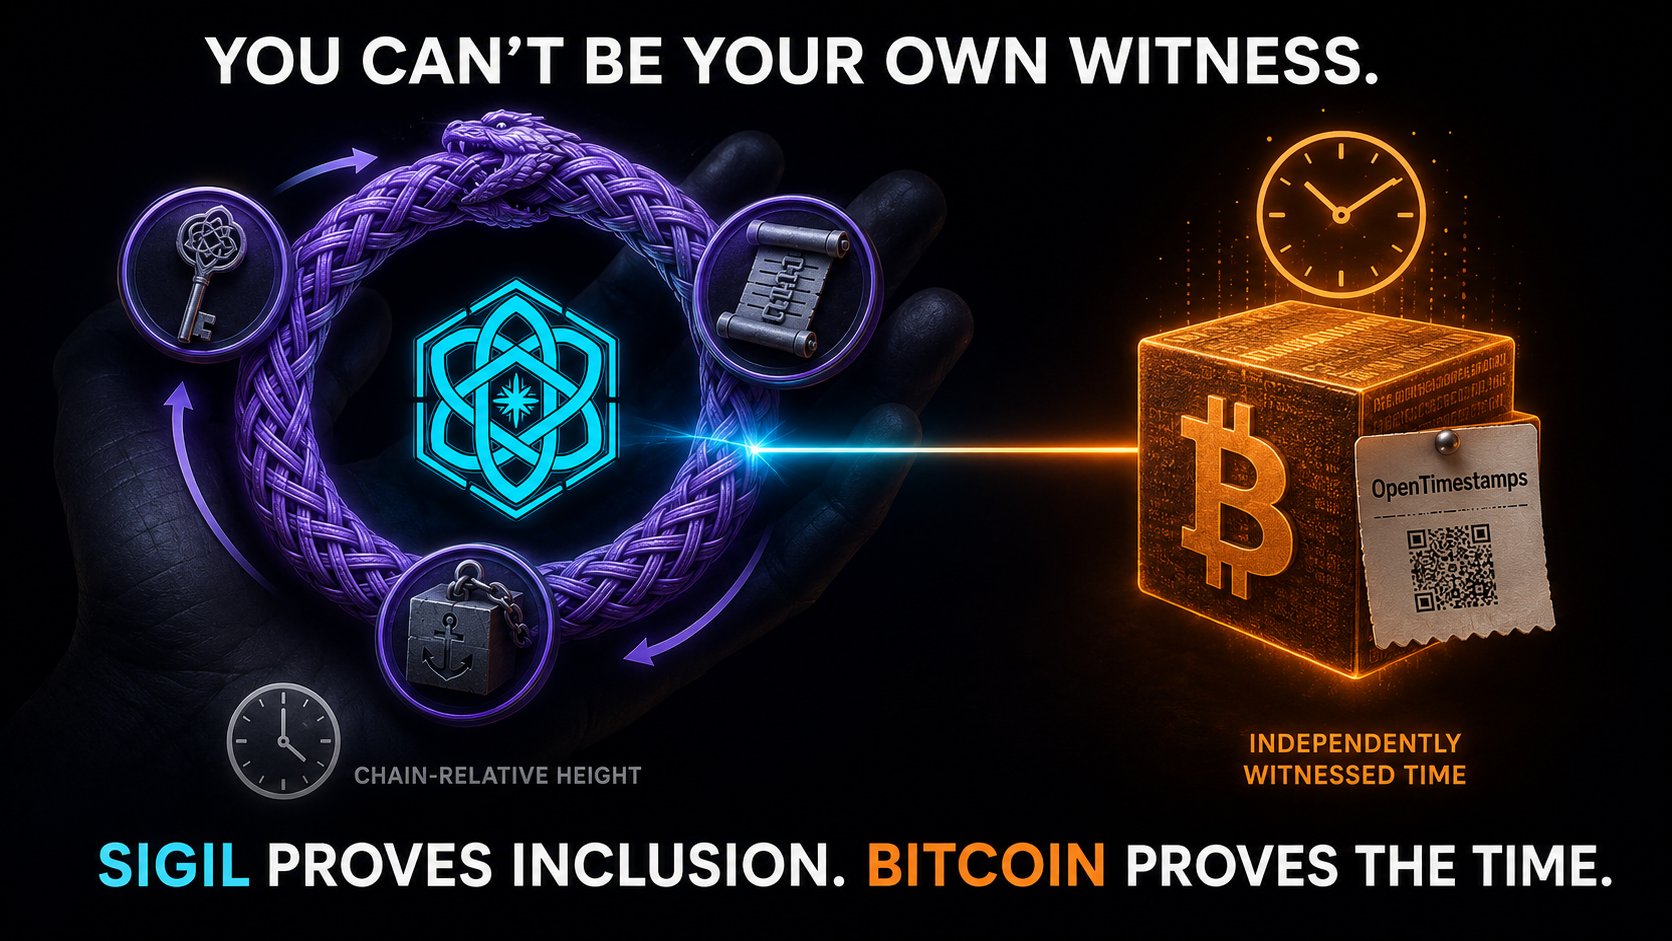
\includegraphics[width=0.60\textwidth]{pro3.png}
\caption{\small One vertical spine, all of it ours: Flux compiler \,$\to$\,
content-addressing \,$\to$\, require-both signing \,$\to$\, the braid / event-log root
\,$\to$\, the fold \,$\to$\, at the cap, a Commitment Record witnessed \emph{inside}
(seal) and \emph{outside} (a Bitcoin receipt). Solid layers are live; dashed layers are
staged --- the honesty is drawn into the diagram.}
\end{figure}

% ============================================================
\section{The Commitment Record}
% ============================================================
A \textbf{Commitment Record} is a canonical statement of intent by the project. Its
fields:

\begin{center}\small
\renewcommand{\arraystretch}{1.25}
\begin{tabularx}{\textwidth}{@{}l l X@{}}
\toprule
\textbf{Field} & \textbf{Type} & \textbf{Meaning} \\
\midrule
\texttt{kind} & enum & \texttt{roadmap} $|$ \texttt{disclosure} $|$ \texttt{release} $|$ \texttt{direction-change} $|$ \texttt{retraction} \\
\texttt{body\_hash} & \texttt{[u8;32]} & BLAKE3 of the exact UTF-8 statement text (the words themselves, stored alongside) \\
\texttt{timestamp\_ms} & u64 & the author's wall clock at signing (informational; the chain height is the trusted time) \\
\texttt{prev} & \texttt{[u8;32]} & content hash of the previous Commitment Record --- the records form their own hash chain \\
\texttt{supersedes} & \texttt{Option<[u8;32]>} & for a \texttt{direction-change}/\texttt{retraction}: the record it revises (never deletes) \\
\texttt{signer\_keys} & pubkeys & the SQIsign-L5 + Ed25519 public keys (pinned, published) \\
\texttt{sig} & bytes & require-both signature over the canonical serialization of all fields above \\
\bottomrule
\end{tabularx}
\end{center}

Two chained structures give it teeth. First, \texttt{prev} makes the records
themselves an append-only hash chain: you cannot silently insert, delete, or reorder a
past commitment without breaking every content hash that follows it. Second, the
record's content hash is emitted as a typed \texttt{CommitmentAnchored} event, so it is
covered by the block's \emph{event-log root} at the height it lands --- and thus by the
header hash, the tip fingerprint, and (below the horizon) the fold. The chain's own
recomputation now witnesses the promise.

Crucially, a \texttt{direction-change} \emph{supersedes} but never erases. Changing
your mind is allowed and expected; doing it \emph{silently} is what the mechanism
forecloses. The old record stays anchored; the new one points back at it. The history
of the project's word becomes a diff, not a palimpsest.

\layman{sigilviolet}{what "supersedes, never deletes" buys}{A project is allowed to
change direction --- honest projects do. What this stops is quietly pretending the old
direction was never promised. The change is recorded as an edit on top of the original,
both permanent, both signed. You can always see what was said first.}

% ============================================================
\section{Verification, a year later}
% ============================================================
A stranger in July 2027, handed a claim of the form \emph{``SIGIL committed in July
2026 that the testnet would be reset before mainnet''}, runs:

\begin{enumerate}[leftmargin=1.4em,itemsep=2pt]
\item \textbf{Recompute the words.} BLAKE3 the statement text; it must equal the
  record's \texttt{body\_hash}. (One byte changed anywhere and this fails.)
\item \textbf{Check the signature.} \texttt{fluxc verify-proof} the require-both
  signature against the \emph{pinned} builder keys --- the same fingerprints already
  published for binaries. A self-consistent record with swapped keys is a forgery and
  is caught exactly as a swapped-key binary proof is.
\item \textbf{Walk the record chain.} Follow \texttt{prev} back; any break means the
  commitment history was tampered with after the fact.
\item \textbf{Confirm the on-chain anchor.} Verify the \texttt{CommitmentAnchored}
  event's inclusion in the event-log root at block height $H$, and $H$ under the tip /
  fold. The chain's own append-only time --- not a server's clock, not a forum's edit
  timestamp --- dates the promise.
\end{enumerate}

If all four pass, the promise \emph{provably existed, in those exact words, signed by
that key, at that height}. If a later public statement contradicts it, the
contradiction is now a checkable fact rather than a memory dispute --- and if the
project revised the commitment properly, step 3 surfaces the \texttt{supersedes} edit
and its own anchor height.

% ============================================================
\section{Independent time: borrowing Bitcoin's clock}\label{sec:time}
% ============================================================
There is a limit the previous sections must not paper over, and it is exactly the one
the original objection targeted. Three different things get proven, and they are not the
same thing: the signature proves \emph{this key attested these exact bytes}; the record
chain proves \emph{these records form a consistent sequence relative to a known head};
and a SIGIL anchor proves \emph{this digest exists at height $H$ in the presently
accepted \texttt{sigil-g0} history}. While \texttt{sigil-g0} is single-producer and
resettable, that third statement is \emph{not} independent calendar time --- the same
authority holds the promise key, the record chain, \emph{and} the anchoring chain, and
could in principle construct a different signed history later. To claim ``provably
existed at that height'' as though it were a witnessed date would overstate precisely
what the reader challenged. Asking SIGIL to certify SIGIL is a circle.

\begin{figure}[h]
\centering
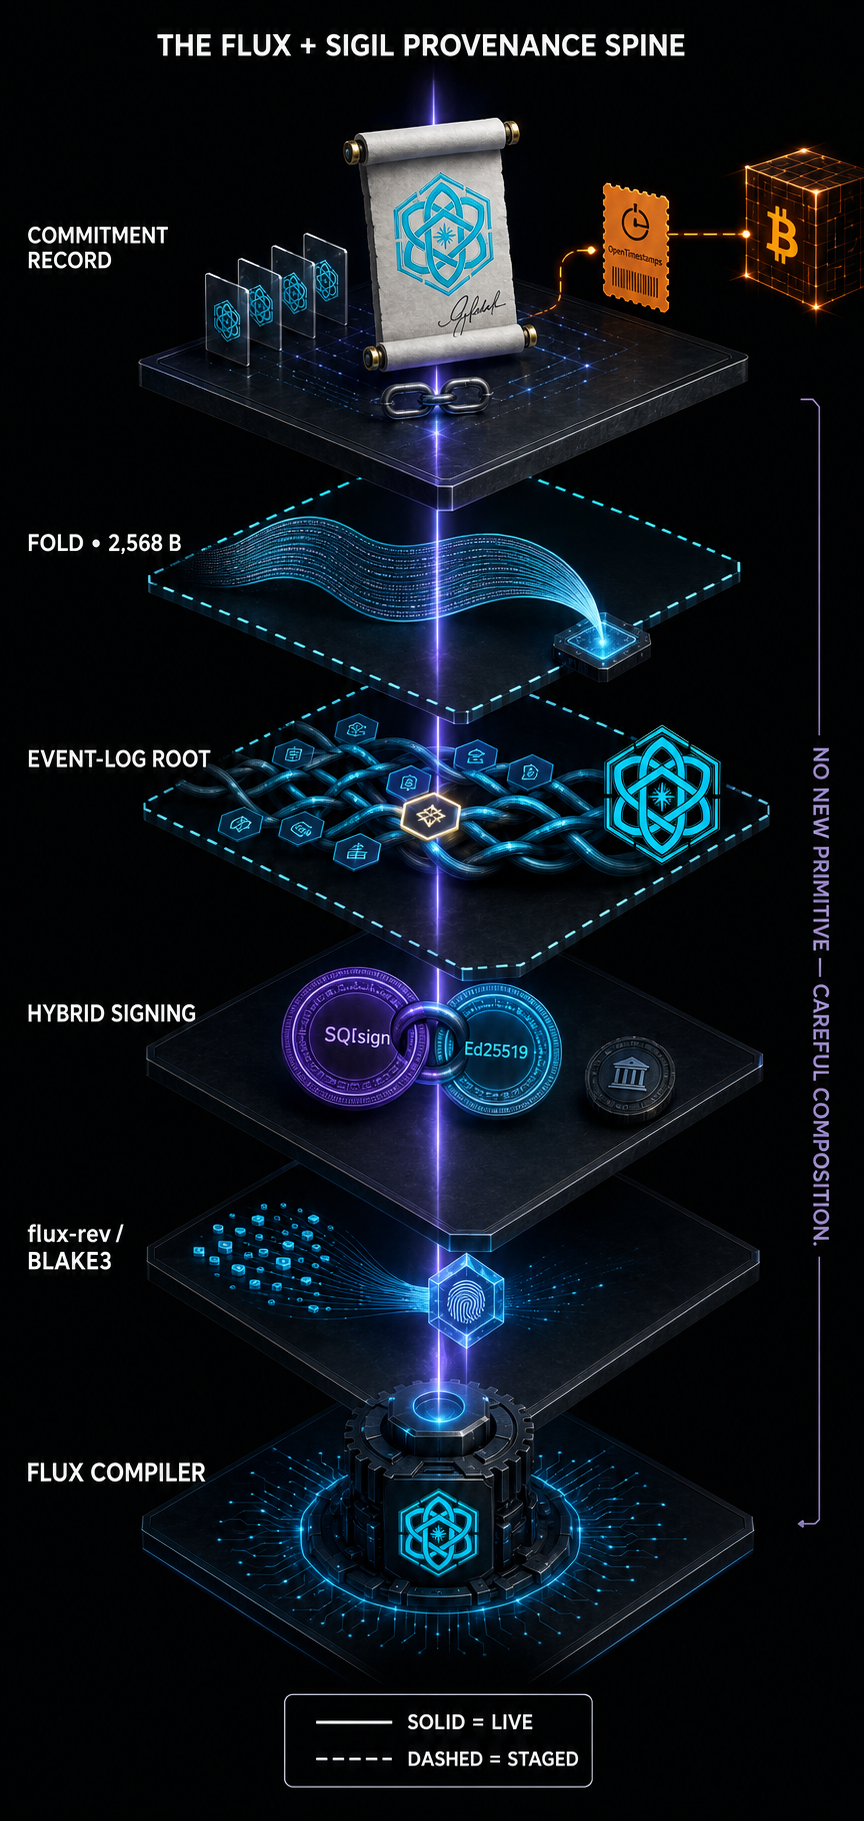
\includegraphics[height=0.42\textheight]{pro2.png}
\caption{\small You cannot be your own witness. The promise key, the record chain, and
the anchoring chain are one hand (the closed \textcolor{sigilviolet}{violet} loop); a
Commitment Record breaks the circle by also stamping onto \textcolor{sigilamber}{Bitcoin}
--- an authority we do not control. SIGIL proves \emph{inclusion}; Bitcoin proves the
\emph{time}.}
\end{figure}

The break in the circle is an external, non-SIGIL witness. Each signed Commitment
Record head is timestamped onto Bitcoin via OpenTimestamps: a proof that the data
existed \emph{no later than} an independently witnessed Bitcoin block, checkable by
anyone with no trust in us. Until SIGIL has an independently operated, non-resettable
producer set, that external timestamp --- not the SIGIL height --- carries the
``no later than'' guarantee; the on-chain anchor \emph{strengthens} as the permissionless
mesh lands. We did not defer this to a promise: \stL~\textbf{this note is itself already
Bitcoin-timestamped}, its receipt published beside it
(\texttt{SIGIL\_COMMITMENT\_PROVENANCE\_v0.pdf.ots}) and verifiable with
\texttt{ots verify}. The best answer to ``how will we know you kept your word'' is a
receipt that already exists, not one we intend to produce.

\layman{sigilamber}{why Bitcoin, of all things}{We can reset our own chain, so a
timestamp only on our chain isn't independent proof of \emph{when} --- we could redo it.
Bitcoin we can't redo. Pinning each promise to a Bitcoin block means the date is
witnessed by something outside our control. That's the difference between a notary who
works for you and one who doesn't.}

% ============================================================
\section{What this does not do (scope, stated plainly)}
% ============================================================
The honesty section is load-bearing here as everywhere in the SIGIL corpus.

\begin{itemize}[leftmargin=1.2em,itemsep=3pt]
\item \stO~\textbf{It does not force a promise to be kept.} It makes a broken or
  edited promise \emph{detectable, dated, and attributable}. Accountability is
  detection plus a permanent record, not enforcement. A project can still break its
  word --- it just can no longer do so \emph{quietly}, and that is the entire aim.
\item \stO~\textbf{It binds a key, not a person.} The signature proves the pinned
  project key attested the statement. Key custody, rotation, and compromise are the
  usual residual trust, identical to the binary-provenance case; the honest posture is
  the same.
\item \stG~\textbf{The anchor's strength tracks the chain's.} Today \texttt{sigil-g0}
  is single-producer and resettable, so an anchor's censorship-resistance is only as
  strong as the network --- which is to say, staged. The record chain (\texttt{prev})
  and the signatures stand \emph{independently} of that, giving tamper-evidence even
  before the chain is adversarial; the on-chain anchor \emph{strengthens} as the
  permissionless multi-producer mesh lands. We label which guarantee is which.
\item \stO~\textbf{It is not yet live.} The event kind, the record schema, and the
  verifier subcommand are specified here and staged in the backlog, not shipped. This
  note claims a design and a first artifact, not a running system --- consistent with
  the project's rule of showing receipts as pieces land, not before.
\end{itemize}

% ============================================================
\section{The recursion, and this note as its seed}
% ============================================================
The pleasing part is the symmetry. SIGIL asks you not to trust its ledger but to
recompute it; this mechanism asks you not to trust its roadmap but to recompute
\emph{that}. The same four-step verification --- recompute the bytes, check the
signature, walk the chain, confirm the anchor --- serves a wallet balance and a
promise alike. The instrument built to hold money to account is turned, without new
machinery, to hold the project's own word to account.

Accordingly, the first Commitment Record the mechanism anchors will be the SIGIL
announcement's own preconditions for mainnet --- the single-producer admission, the
no-allocation statement, the named hardening list, the reset-before-mainnet pledge ---
signed and content-addressed, so that the promises this project is judged by are, from
the start, the promises this project cannot later revise in silence. This note is
offered as the seed of that record. The reader who asked the question will, by design,
be able to check that we kept it.

\vspace{8pt}
\begin{center}\small\itshape\textcolor{gray}{%
Origin: this note answers a question raised by \texttt{fibonacciopstan} on
BitcoinTalk. That a community reader defined the requirement, and that the project
records the requirement's origin here, is itself the accountability the note is about.}
\end{center}

\end{document}
